%%%%%
%%%%%  Use LUALATEX, not LATEX.
%%%%%
%%%%
\documentclass[]{VUMIFTemplateClass}

\usepackage{indentfirst}
\usepackage{amsmath, amsthm, amssymb, amsfonts}
\usepackage{mathtools}
\usepackage{physics}
\usepackage{graphicx}
\usepackage{verbatim}
\usepackage[hidelinks]{hyperref}
\usepackage{xcolor,algorithm,algorithmic}
\definecolor{gray}{gray}{0.6}


\usepackage{tcolorbox}

\newcommand{\yellowcomment}[1]{%
    \begin{tcolorbox}[colback=yellow!80, colframe=yellow!80, arc=0pt, outer arc=0pt, boxrule=0pt, left=3pt, right=3pt, top=3pt, bottom=3pt]
        \textbf{\textcolor{red}{COMMENT:}} #1
    \end{tcolorbox}
}

\newcommand{\warningcomment}[1]{%
    \begin{tcolorbox}[colback=yellow!90, colframe=red, arc=0pt, outer arc=0pt, boxrule=2pt, left=5pt, right=5pt, top=5pt, bottom=5pt]
        \Large\textbf{\textcolor{red}{FIX THIS: }} \normalsize #1
    \end{tcolorbox}
}

\newcommand{\goodcomment}[1]{%
    \begin{tcolorbox}[colback=green!20, colframe=green!60, arc=0pt, outer arc=0pt, boxrule=1pt, left=3pt, right=3pt, top=3pt, bottom=3pt]
        \textbf{\textcolor{green!70!black}{GOOD:}} #1
    \end{tcolorbox}
}

\newcommand{\noticecomment}[1]{%
    \begin{tcolorbox}[colback=blue!20, colframe=blue!60, arc=0pt, outer arc=0pt, boxrule=1pt, left=3pt, right=3pt, top=3pt, bottom=3pt]
        \textbf{\textcolor{blue!70!black}{NOTE:}} #1
    \end{tcolorbox}
}

\newcommand{\todocomment}[1]{%
    \begin{tcolorbox}[colback=red!20, colframe=red!60, arc=0pt, outer arc=0pt, boxrule=1pt, left=3pt, right=3pt, top=3pt, bottom=3pt]
        \textbf{\textcolor{orange!70!black}{TODO:}} #1
    \end{tcolorbox}
}

\newcommand{\suggestioncomment}[1]{%
    \definecolor{lime}{RGB}{50,205,50}%
    \begin{tcolorbox}[colback=lime!15, colframe=lime!60, arc=0pt, outer arc=0pt, boxrule=1pt, left=3pt, right=3pt, top=3pt, bottom=3pt]
        \textbf{\textcolor{lime!70!black}{SUGGESTION:}} #1
    \end{tcolorbox}%
}

\usepackage[nottoc]{tocbibind}
\usepackage{tocloft}
\usepackage{longtable}
\usepackage{amssymb}

\usepackage{titlesec}
\newcommand{\sectionbreak}{\clearpage}

\makeatletter
\renewcommand{\fnum@algorithm}{\thealgorithm}
\makeatother
\renewcommand\thealgorithm{\arabic{algorithm} algorithm}

\usepackage{biblatex}
\bibliography{bibliografija}
%% to change the numbering (numeric or alphabetic) of bibliographic sources, make the change in VUMIFTemplateClass.cls, line 139

% Author's MACROS
\newcommand{\EE}{\mathbb{E}\,} % Mean
\newcommand{\ee}{{\mathrm e}}  % nice exponent
\newcommand{\RR}{\mathbb{R}}

\makeatletter
% introduce a 4th-level sectioning command: \subsubsubsection
\newcounter{subsubsubsection}[subsubsection]
\renewcommand\thesubsubsubsection{\thesubsubsection.\arabic{subsubsubsection}}

\providecommand\subsubsubsection{%
    \@startsection{subsubsubsection}{4}{\z@}%
        {-3.25ex\@plus -1ex \@minus -.2ex}%
        {1.5ex \@plus .2ex}%
        {\normalfont\normalsize\bfseries}%
}

% ensure numbering and TOC include this level
\setcounter{secnumdepth}{4}
\setcounter{tocdepth}{4}
\makeatother


\studyprogramme{Software Engineering} %Write your study programme (example – Software engineering, Financial and Actuarial Mathematics, etc.)
\worktype{PS Software Design} % Bachelor's thesis or Master's thesis
\worktitle{PS Sofware Design documentation}
% \secondworktitle{Work Title in Lithuanian}
\workauthor{Tadas Riksas, Darius Spruogis, Gustas Mickus, Julius Jauga}

%There may be more than one author, in which case each author is written from a new line which is added in Titlepage.tex or LongerTitlePage.tex
%\secondauthor{Name Surname} %If present, otherwise delete

\supervisor{Vasilij Savin}
% \reviewer{pedagogical/scientific title Name Surname} %If present, otherwise delete
% \scientificadvisor{pedagogical/scientific title Name Surname} %If present, otherwise delete

\begin{document}
\selectlanguage{english}

\onehalfspacing
\begin{titlepage}
\vskip 20pt
\begin{center}

\includegraphics[scale=0.55]{images/MIF.png}
\end{center}

\makeatletter

\vskip 20pt
\centerline{\bf \large \textbf{VILNIUS UNIVERSITY}}
\vskip 10pt
\centerline{\large \textbf{FACULTY OF MATHEMATICS AND INFORMATICS}}
\vskip 10pt
\centerline{\large \textbf{\MakeUppercase{\@studyprogramme \space study programme}}}

\vskip 80pt
\centerline{\Large \@worktype}
\vskip 20pt
\begin{center}
    {\bf \LARGE \@worktitle}
\end{center}
\begin{center}
    {\bf \Large \@secondworktitle}
\end{center}
\vskip 80pt

\centering{\Large \@workauthor}
\@ifundefined{@secondauthor}{}
{
\vskip 10pt
\centering{\Large \@secondauthor}
}
\vskip 20pt

\centering{
    \begin{tabular}{rcp{.7\textwidth}}
        {\Large Supervisor} & {\Large :} & {\Large \@supervisor}\\[10pt]
        \@ifundefined{@scientificadvisor}{}
            {
                {\Large Scientific advisor} & {\Large :} & {\Large \@scientificadvisor}\\[10pt]
            }
        \@ifundefined{@reviewer}{}
            {
                {\Large Reviewer} & {\Large :} & {\Large \@reviewer}\\[10pt]
            }
    \end{tabular}}


\vskip 110pt

\centerline{\large \textbf{Vilnius}}
\centerline{\large \textbf{\the\year{}}}

\makeatother

\newpage
\end{titlepage}
%\newgeometry{top=2cm,bottom=2cm,right=2cm,left=3cm}
\setcounter{page}{2}


\tableofcontents
\onehalfspacing


\section*{Check list \checkmark}

The suggested structure below is only a recommendation. You can decide to adopt a different flow as long as you cover everything that is relevant for the system under design. One good way of testing it is to designate one person on the team who will take on an implementer's hat and read through the document as if they will have to implement that document.

\begin{enumerate}
    \item Intro
    \item Business flows (with sequence diagrams or flow diagrams)
    \item Package diagrams showing classes/modules of the system - high level architecture
    \item Data model for entity used in the system (recommended class diagrams instead of ER diagrams)
    \item API Contracts for the backend endpoints (with Swagger/Open API)
    \begin{itemize}
        \item HTTP requests with all possible parameters
        \item HTTP responses
        \item HTTP error codes
    \end{itemize}
\end{enumerate}

\subsection*{Submission Requirements}

The team will have to prepare two documents:

\begin{itemize}
    \item \textbf{A shared text document} with all diagrams, descriptions and other relevant technical details needed. This document is shared with the lecturer and the final snapshot past submission deadline will be used for grading. You can use Word, Google Docs or Overleaf to share this document.
    
    \item \textbf{A plaintext document in YAML format} that can be loaded into \href{https://editor.swagger.io/}{https://editor.swagger.io/}. This document is put into your team's repository and the link to your Git repo is provided by the team lead to lecturer.
\end{itemize}

It is expected that your YAML file should load there without syntax errors. If the upload fails, only the visible parts of API Design will be graded.

\subsection*{System-under-design Business Requirements}

We are simulating a Software as a Service startup that you will be running. You are creating software for small and medium businesses in catering (bars/cafe/restaurants) and beauty (barbers/hairdressers/SPA) sectors. Your system needs to support both functionalities; however, feature sets can be regulated by the plan your customers subscribed to.

It is enough to design system that is only operated by business employees where the only input customer provides is payment and contact information for bookings.

This list can be expanded/clarified by additional questions raised by students during the design process. It is not meant to be a complete list from the get-go.

\subsubsection*{Order Functionality}

\begin{itemize}
    \item Employee can create an order
    \item Employee can modify an open order (change items)
    \item Employee cannot modify a closed/paid order
    \item Employee can cancel an open (unpaid/not closed order)
    \item Customer can pay the order by cash, gift card and credit/debit card
    \begin{itemize}
        \item \textbf{BEWARE:} In Lab 2 every team will be asked to implement card payment integration with Stripe payment provider, so you might want to do extra research on how card payment flow works.
    \end{itemize}
    \item Each order should allow split checks (multiple payments).
    \item Customer can add a tip to an order.
    \item Employee can apply a discount to an order.
    \item When order is closed the customer can get the final receipt with all costs, taxes, discounts and service charges calculated and presented
    \begin{itemize}
        \item Different order items can have different taxes applied to them (food vs alcohol as an example)
    \end{itemize}
    \item Paid/closed orders are to be preserved indefinitely.
    \item Closed orders can be refunded and marked as such.
\end{itemize}

\subsubsection*{Services}

\begin{itemize}
    \item Employee can make a reservation for a customer
    \begin{itemize}
        \item Each reservation has time when booked, appointment time, employee, customer, service
    \end{itemize}
    \item Employee can cancel or modify an appointment upon customer request
    \item \textbf{BONUS} - send SMS notification when appointment is created (I recommend AWS SMS functionality for that)
\end{itemize}

\subsubsection*{System Management Functionality}

\begin{itemize}
    \item \textbf{BONUS:} Inventory management (should be integrated with order management and have quantities reduced when bought)
    \item Tax Management (create/edit/delete)
    \begin{itemize}
        \item Change of the tax entry (like VAT) should not affect any historical records
    \end{itemize}
    \item Service charge/Tip/Gratuity Management
    \begin{itemize}
        \item Change of the service charge item should not affect any historical records
    \end{itemize}
    \item Product/Menu Item Management (create/edit/delete)
    \item Each product can have variations (e.g. coffee with milk, decaf, vegan milk)
    \item Each Service has an employee associated with it
    \item Discount Management
    \begin{itemize}
        \item Discounts can be applied to a specific product or the whole order
        \item Discounts can be time-limited
    \end{itemize}
    \item User Management (can create/delete/edit users)
    \begin{itemize}
        \item Only business owner can edit employees/users of their business
        \item SuperAdmin (IT Support) can edit anyone
        \item All actions should be performed only by logged-in and authorized users
    \end{itemize}
    \item Merchant/Business management
    \begin{itemize}
        \item Each merchant/business has an owner user, address, contact info (phone, email), name and other relevant details
    \end{itemize}
\end{itemize}


%% Acknowledgements Section
\sectionnonumnocontent{Acknowledgements}
The author is thankful to the lecturer Vasilij Savin for his guidance and
support throughout the project.


% Lets first give some context to copilot
% #  **Business Management System - Project Summary**

% ##  **Project Overview**
% Building a **multi-tenant SaaS platform** for small service businesses (bars, restaurants, spas, salons) to manage their operations, appointments, orders, and payments in one unified system.

% ##  **Core Business Domains**

% ### ️ **Order Management** (Bars/Restaurants)
% - **Table-based ordering** with real-time modifications
% - **Split bills**, tips, discounts, and multiple payment methods
% - **Menu management** with item variations (e.g., coffee types, milk options)
% - **Inventory tracking** and stock management

% ###  **Services Management** (Spas/Salons)  
% - **Appointment scheduling** with time slot booking
% - **Employee availability** and conflict prevention
% - **Service catalog** (massages, haircuts, treatments)
% - **SMS notifications** for confirmations and reminders

% ## ️ **Technical Requirements**

% ### **Multi-tenancy Architecture**
% - Single database supporting **multiple businesses**
% - Data isolation between different business tenants
% - Super admin access for system management

% ### **Data Model Criticalities**
% - **Historical data preservation** (price/tax changes must NOT affect past records)
% - **Soft deletion** instead of physical data removal
% - **Calculated fields** handled in application layer, not database

% ### **Key Integration Points**
% - **Payment processing** (Stripe integration)
% - **SMS gateway** for appointment notifications
% - **Role-based authentication** (Customer, Employee, Manager, Admin)

% ##  **Current Focus: Business Flow Division**
% We're analyzing and documenting business workflows across **4 functional domains**:
% 1. **Core Service Delivery & Booking**
% 2. **Customer & Business Management** 
% 3. **Communication & Operations**
% 4. **Payments & Analytics**

% ##  **Academic Context**
% This is for a **software design course** where we're creating technical specifications before implementation. The project emphasizes **proper documentation, data modeling, and API design** following software engineering best practices.

% ##  **Current Task**
% Dividing business flow documentation among team members while maintaining **consistency, clear boundaries, and minimal dependencies** between work streams.

% ---
% **Key Constraint:** The system must handle **both order-based (restaurants) and appointment-based (spas) businesses** with overlapping but distinct workflows.


\section{Introduction}
This document outlines the software design for a multtenant SaaS platform
aimed at small to medium business that consentrate on order delivery such as
bars, restaurants and services such as spas and salons. The platform will
provide a unified system for managing operations, appointments, orders, and
payments.


% ========================================================================
% FUNCTIONAL DOMAIN SEPARATION
% ========================================================================

% ------------------------------------------------------------------------
% DOMAIN INTERACTIONS
% ------------------------------------------------------------------------

% RESTAURANT ↔ MANAGEMENT
% - Employee assignments to tables/shifts
% - Financial data aggregation
% - Customer profile updates

% SERVICES ↔ MANAGEMENT
% - Employee scheduling and availability
% - Appointment revenue tracking
% - Customer service history

% RESTAURANT ↔ SERVICES (for hybrid businesses)
% - Shared customer profiles
% - Combined service packages
% - Unified payment processing

% NOTE: This separation allows each domain to be developed independently
% while maintaining clear integration points for businesses that operate
% across multiple domains.

\section{Business Flows}

We will first start with business flows by describing the business process we are automating. We will
seperate the business flows into 3 main domains for clarity:
\begin{itemize}
    \item Order Management (Bars/Restaurants)
    \item Services Management (Spas/Salons)
    \item Business Management
\end{itemize}
These domains will communicate in this simple way:
\begin{itemize}
    \item Order Management <-> Business Management
    \item Services Management <-> Business Management
\end{itemize}

We will try to write the business flows and then identify the entities,
components and actions needed to implement these business flows.

% example of how to analyze a business flow
% Autoshop business flow

%     • Client arrives at the autoshop
%     • Mechanic engages new client and asks about the reason for the visit
%     • Client fills in the intake form (contact info, car plates, VIN, complaints/issues, etc)
%     • Mechanic gives initial estimate for time and cost of the fix
%     • Client accepts the quote and gives car keys to the mechanic
%     • Mechanic moves car to the parking lot for cars awaiting repairs
%     • Mechanic initiates repairs (possible uncovering additional issues)
%     • Mechanic orders required spare parts OR Mechanics retrieves needed parts from storage
%     • Mechanic contacts client and provides new estimate for cost and time of repairs
%     • Client approves the update quote
%     • Mechanic completes the repairs
%     • Mechanic moves car to the parking lot of cars awaiting pick up.
%     • Client arrives, pays for the repairs and departs
%     • Mechanic adds closing notes to the fix order and closes the order

% Tables/Entities
% Car
% Employee
% Service? Repair Type performed
% Repairs by order
% Spare parts
% Autoshop
% Inventory

% Components
% Order Management (Order, Payments)
% Employee Management
% Inventory (Spare parts, Inventory)
% Catalogue/Offering (Service? Repair Type performed, Repairs by order)


% Actions
% Client fills in the intake form
% Client accepts the quote
% Client approves the update quote
% Client pays for the repairs


\subsection{Order Management (Bars/Restaurants)}

% ------------------------------------------------------------------------------
% ORDER DOMAIN
% (Related to bars, restaurants, cafes — places where customers place orders for items like food and drinks)
%
% Use Case          | Description
% ------------------|--------------------------------------------------------------------
% Create Order      | Employee creates a new order for a customer (e.g., at a table).
% Modify Order      | Add, remove, or update items in an open order.
% Close Order       | Finalize the order when the customer is done.
% Pay Order         | Process payment (cash, card, gift card, split payment).
% Apply Discount    | Specify discounts can be applied to specific products OR entire orders
% Add Tip           | Allow the customer to add a tip to the bill.
% Cancel Order      | Cancel an open order before payment.
% Refund Order      | Process a refund for a paid order (e.g., due to complaint).
% Print Receipt     | Generate a final receipt with items, taxes, discounts, and totals.
% Split Check       | Split the bill among multiple customers.
% Handle Different Tax Rates per Item | Apply different tax rates (e.g., food vs. alcohol).
% Refund Order      | Process refund for closed/paid orders and mark them as refunded.
% Preserve Historical Orders | Keep closed/paid orders indefinitely without modification
% ------------------------------------------------------------------------------


\begin{longtable}{p{0.25\linewidth} p{0.70\linewidth}}
\caption{Use cases for the Order Management domain} \\
\textbf{Use case} & \textbf{Description} \\
\hline
\endfirsthead

\multicolumn{2}{c}{{\tablename\ \thetable{} -- Continued from previous page}} \\
\textbf{Use case} & \textbf{Description} \\
\hline
\endhead

\multicolumn{2}{c}{{Continued on next page}} \\
\endfoot

\endlastfoot

Client Seating (Available) &
\begin{minipage}[t]{\linewidth}
Employee checks seating via POS \& backend. If available, employee assigns a table and confirms with client.
\end{minipage} \\[6pt]
\multicolumn{2}{@{}c@{}}{\color{gray}\rule{0.95\linewidth}{0.4pt}} \\[6pt]

Client Seating (Not Available) &
\begin{minipage}[t]{\linewidth}
Employee checks seating via POS \& backend, finds no seats available, and informs client.
\end{minipage} \\[6pt]
\multicolumn{2}{@{}c@{}}{\color{gray}\rule{0.95\linewidth}{0.4pt}} \\[6pt]

Place Order &
\begin{minipage}[t]{\linewidth}
Client requests menu, places an order via employee. POS \& backend validate items, stock, and combinations. If valid, client confirms; else corrections are requested.
\end{minipage} \\[6pt]
\multicolumn{2}{@{}c@{}}{\color{gray}\rule{0.95\linewidth}{0.4pt}} \\[6pt]

Modify Order &
\begin{minipage}[t]{\linewidth}
Client requests to update an existing order. Employee updates through POS, backend validates. On success, order is updated; on failure, errors are shown for correction.
\end{minipage} \\[6pt]
\multicolumn{2}{@{}c@{}}{\color{gray}\rule{0.95\linewidth}{0.4pt}} \\[6pt]

Cancel Order &
\begin{minipage}[t]{\linewidth}
Client requests to cancel an existing not completed order. Employee cancels through POS, backend validates that it is not completed. On success, order is updated; on failure, errors are shown.
\end{minipage} \\[6pt]
\multicolumn{2}{@{}c@{}}{\color{gray}\rule{0.95\linewidth}{0.4pt}} \\[6pt]

Mark items as delivered for table &
\begin{minipage}[t]{\linewidth}
The employee selects a table. The order with items are retrieved for that table, which is then displayed in the POS. The employee selects items to mark as delivered. The item status is updated in the backend server, and a confirmation is displayed in the POS.
\end{minipage} \\[6pt]
\multicolumn{2}{@{}c@{}}{\color{gray}\rule{0.95\linewidth}{0.4pt}} \\[6pt]

\end{longtable}



\subsection{Services Management (Spas/Salons)}

% ------------------------------------------------------------------------------
% Service Domain
% (Related to appointment-based businesses like spas, barbers, massage centers)
%
% Use Case             | Description
% ---------------------|-----------------------------------------------------------------
% Create Appointment   | Employee schedules a service for a customer (date, time, employee).
% Modify Appointment   | Change time, employee, service, date, or assigned employee.
% Cancel Appointment   | Cancel a scheduled service.
% Check Availability   | Verify if an employee is free at a given time.
% Send SMS Reminder    | Automatically send an SMS to the customer before the appointment.
% Assign Employee      | Assign a specialist to a service.
% Mark Service as Done | Record that the service has been completed.
% ------------------------------------------------------------------------------


We have identified the following use cases for the services management domain:

\vspace{1cm}
\begin{longtable}{p{0.25\linewidth} p{0.70\linewidth}}
\caption{Use cases for the Services Management domain} \\
\textbf{Use case} & \textbf{Description} \\
\hline
\endfirsthead

\multicolumn{2}{c}{{\tablename\ \thetable{} -- Continued from previous page}} \\
\textbf{Use case} & \textbf{Description} \\
\hline
\endhead

\multicolumn{2}{c}{{Continued on next page}} \\
\endfoot

\endlastfoot

Create appointment &
\begin{minipage}[t]{\linewidth}
Employee or customer schedules a service for a customer by selecting service, date/time and (optionally) employee; system reserves the slot, records booking metadata and sends confirmation.
\end{minipage} \\[6pt]
\multicolumn{2}{@{}c@{}}{\color{gray}\rule{0.95\linewidth}{0.4pt}} \\[6pt]

Modify appointment &
\begin{minipage}[t]{\linewidth}
Change appointment details (time, service, date, assigned employee); system validates availability, preserves historical record of changes and notifies affected parties.
\end{minipage} \\[6pt]
\multicolumn{2}{@{}c@{}}{\color{gray}\rule{0.95\linewidth}{0.4pt}} \\[6pt]

Cancel appointment &
\begin{minipage}[t]{\linewidth}
Customer or staff cancels an appointment; system frees the slot, applies cancellation rules (refund/deposit handling if applicable) and sends notifications.
\end{minipage} \\[6pt]
\multicolumn{2}{@{}c@{}}{\color{gray}\rule{0.95\linewidth}{0.4pt}} \\[6pt]

% Check availability &
% \begin{minipage}[t]{\linewidth}
% Verify employee and resource availability for requested time considering working hours, breaks and existing bookings; support searching for next available slots and preventing double-booking.
% \end{minipage} \\[6pt]
% \multicolumn{2}{@{}c@{}}{\color{gray}\rule{0.95\linewidth}{0.4pt}} \\[6pt]

% Send SMS reminder &
% \begin{minipage}[t]{\linewidth}
% Schedule and send SMS/email reminders (configurable templates and timing) before appointments; include retry and failure handling and opt‑out management.
% \end{minipage} \\[6pt]
% \multicolumn{2}{@{}c@{}}{\color{gray}\rule{0.95\linewidth}{0.4pt}} \\[6pt]

% Assign employee &
% \begin{minipage}[t]{\linewidth}
% Map employees to services they can perform and assign staff to bookings either manually or automatically based on skills and availability; support reassignment workflows.
% \end{minipage} \\[6pt]
% \multicolumn{2}{@{}c@{}}{\color{gray}\rule{0.95\linewidth}{0.4pt}} \\[6pt]

Service Customer &
\begin{minipage}[t]{\linewidth}
    The customer gets the service done by the assigned employee; employee marks the service as completed in the system, which updates records and triggers any follow-up actions (e.g., feedback request, payment processing).
\end{minipage} \\
\end{longtable}

\vspace{1cm}


\subsubsection{Appointment creating business flow}

Flow:
\begin{itemize}
    \setlength{\itemsep}{2pt}
    \setlength{\parskip}{0pt}
    \setlength{\parsep}{0pt}
    \item Customer calls or walks in to the spa/salon
    \item Customer meets with the employee
    \item Customer requests a service
    \item Employee checks availability of the requested service
    \item If available, the employee asks when the customer would like to book the service
    \item Customer provides a date and time
    \item Employee checks availability for the requested date and time
    \item If available, employee asks if the customer has a preference for a specific employee
    \item Customer provides a preference (or not)
    \item Employee checks availability of the requested employee (if any)
    \item Employee asks for customer contact information (phone number, email)
    \item Customer provides contact information
    \item Employee creates the appointment in the POS system
    \item System sends a confirmation SMS/email to the customer
\end{itemize}

Tables/Entities:
\begin{itemize}
    \setlength{\itemsep}{2pt}
    \setlength{\parskip}{0pt}
    \setlength{\parsep}{0pt}
    \item Customer
    \item Employee
    \item Service
    \item Appointment
    \item Spa/Salon (Business)
\end{itemize}

Components:
\begin{itemize}
    \setlength{\itemsep}{2pt}
    \setlength{\parskip}{0pt}
    \setlength{\parsep}{0pt}
    \item Appointment Management (Appointment, Employee, Service)
    \item Employee Management (Employee)
    \item Notification System (SMS/Email)
\end{itemize}

Actions:
\begin{itemize}
    \setlength{\itemsep}{2pt}
    \setlength{\parskip}{0pt}
    \setlength{\parsep}{0pt}
    \item Check availability of service
    \item Check availability of employee
    \item Create appointment
    \item Send confirmation notification
\end{itemize}

\begin{figure}[H]
    \centering
    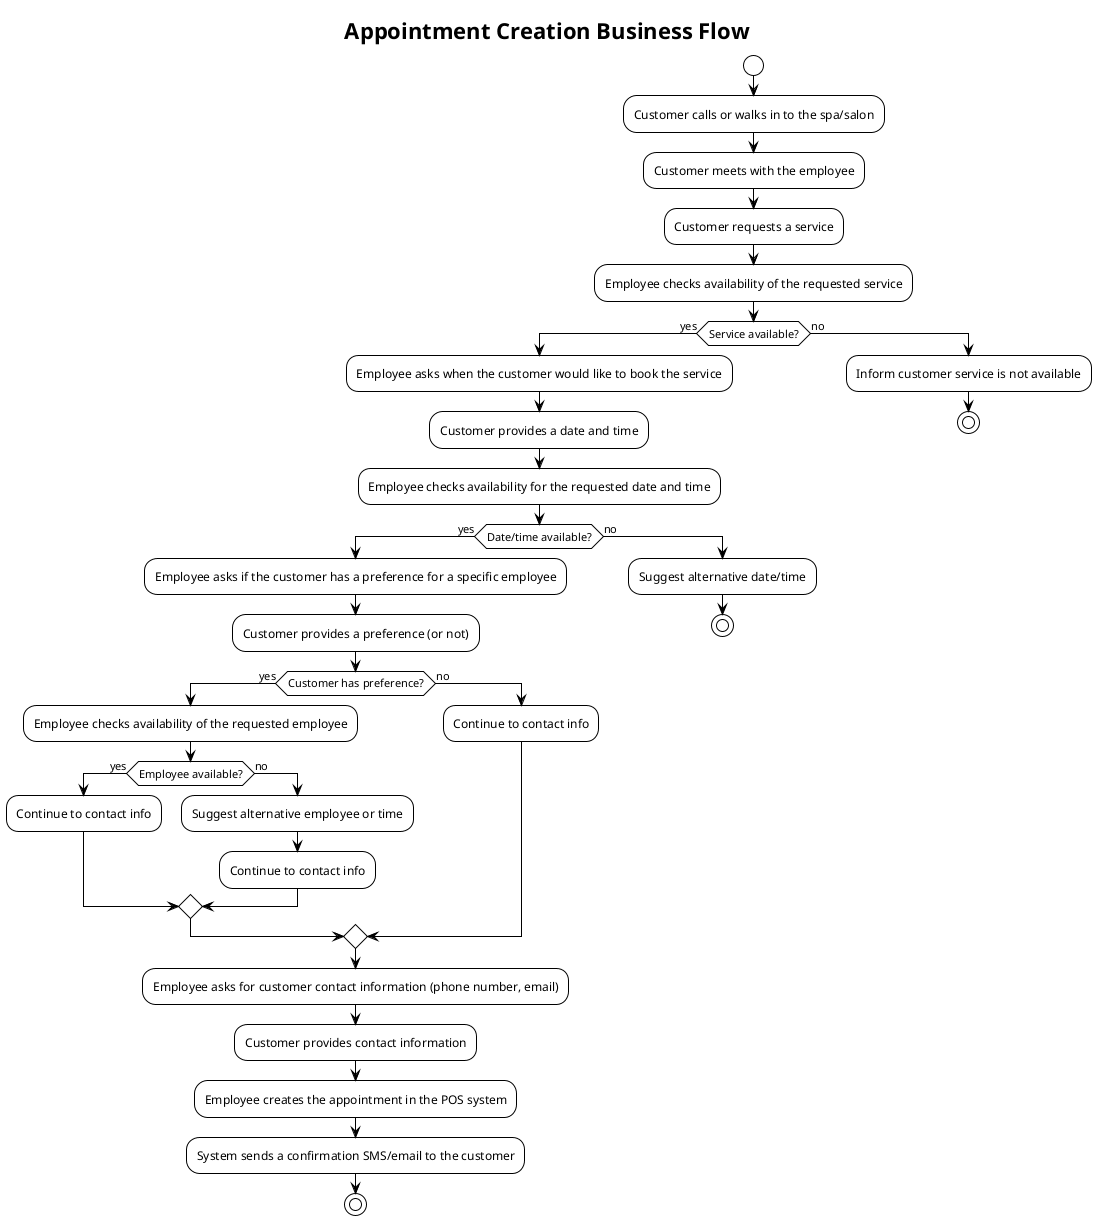
\includegraphics[width=0.8\textwidth]{images/diagrams/services/appointment_creation_flow.png}
    \caption{Appointment Creation Flow Diagram}
    \label{fig:appointment_creation_flow}
\end{figure}

\begin{figure}[H]
    \centering
    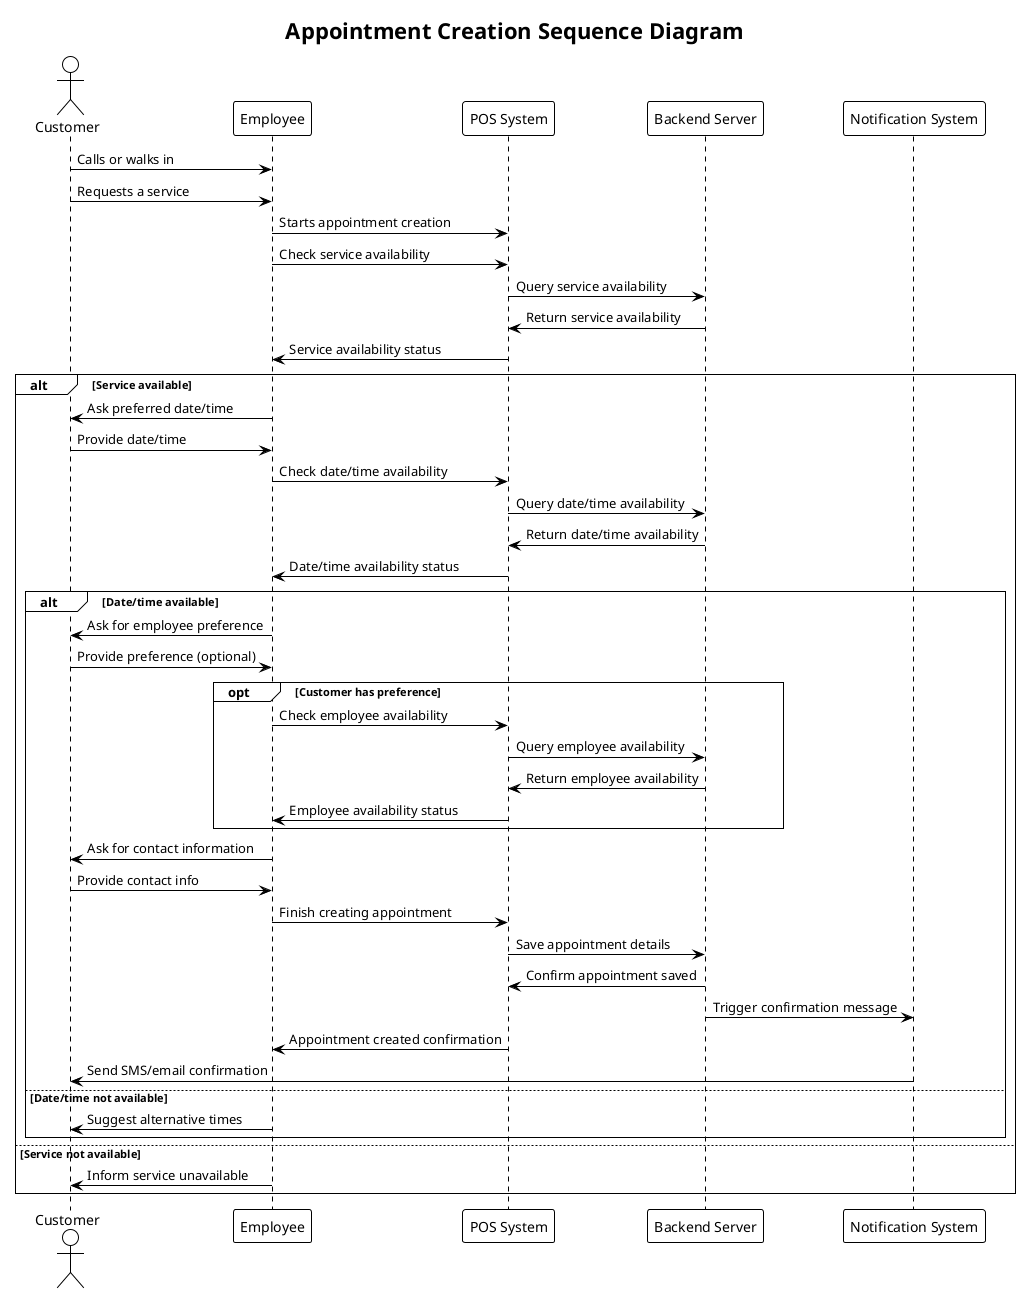
\includegraphics[width=0.8\textwidth]{images/diagrams/services/appointment_creation_sequence.png}
    \caption{Appointment Creation Sequence Diagram}
    \label{fig:appointment_creation_sequence}
\end{figure}

\subsubsection{Appointment modification business flow}

Flow:
\begin{itemize}
    \setlength{\itemsep}{2pt}
    \setlength{\parskip}{0pt}
    \setlength{\parsep}{0pt}
    \item Customer calls or walks in to the spa/salon
    \item Customer meets with the employee
    \item Customer requests to modify an existing appointment
    \item Employee asks for customer contact information (phone number, email)
    \item Customer provides contact information
    \item Employee retrieves the appointment using the provided contact information
    \item Employee discusses the requested changes with the customer (date, time, service, employee)
    \item Employee checks availability for the requested changes
    \item If available, employee updates the appointment in the POS system
    \item System sends an updated confirmation SMS/email to the customer
\end{itemize}

Tables/Entities:
\begin{itemize}
    \setlength{\itemsep}{2pt}
    \setlength{\parskip}{0pt}
    \setlength{\parsep}{0pt}
    \item Customer
    \item Employee
    \item Service
    \item Appointment
    \item Spa/Salon (Business)
\end{itemize}

Components:
\begin{itemize}
    \setlength{\itemsep}{2pt}
    \setlength{\parskip}{0pt}
    \setlength{\parsep}{0pt}
    \item Appointment Management (Appointment, Employee, Service)
    \item Employee Management (Employee)
    \item Notification System (SMS/Email)
\end{itemize}

Actions:
\begin{itemize}
    \setlength{\itemsep}{2pt}
    \setlength{\parskip}{0pt}
    \setlength{\parsep}{0pt}
    \item Retrieve appointment
    \item Check availability of service
    \item Check availability of employee
    \item Update appointment
    \item Send updated confirmation notification
\end{itemize}

\begin{figure}[H]
    \centering
    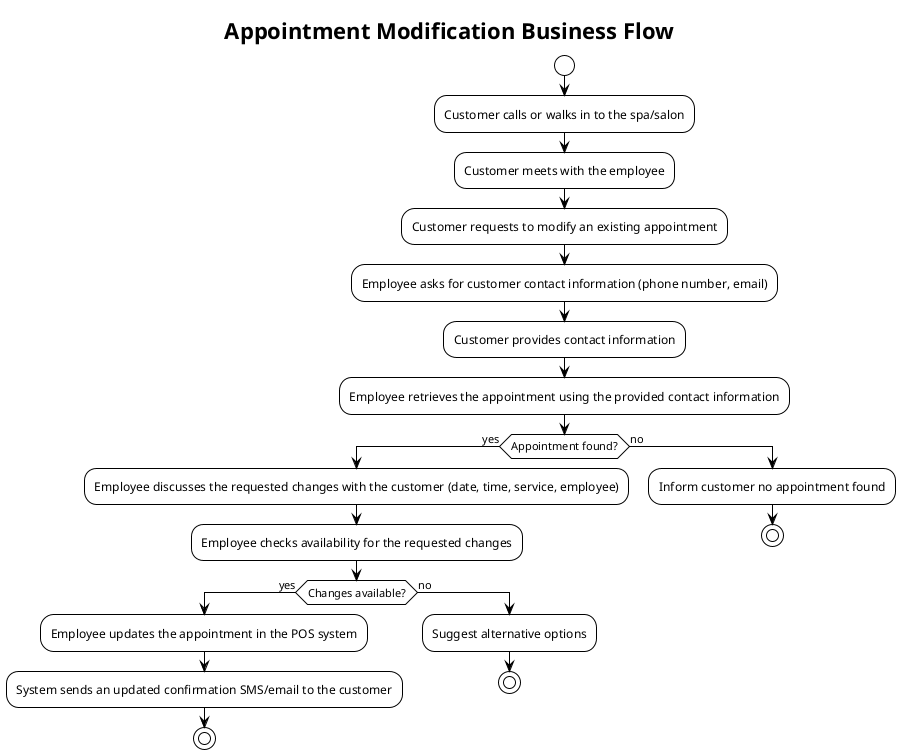
\includegraphics[width=0.8\textwidth]{images/diagrams/services/appointment_modification_flow.png}
    \caption{Appointment Modification Flow Diagram}
    \label{fig:appointment_modification_flow}
\end{figure}

\begin{figure}[H]
    \centering
    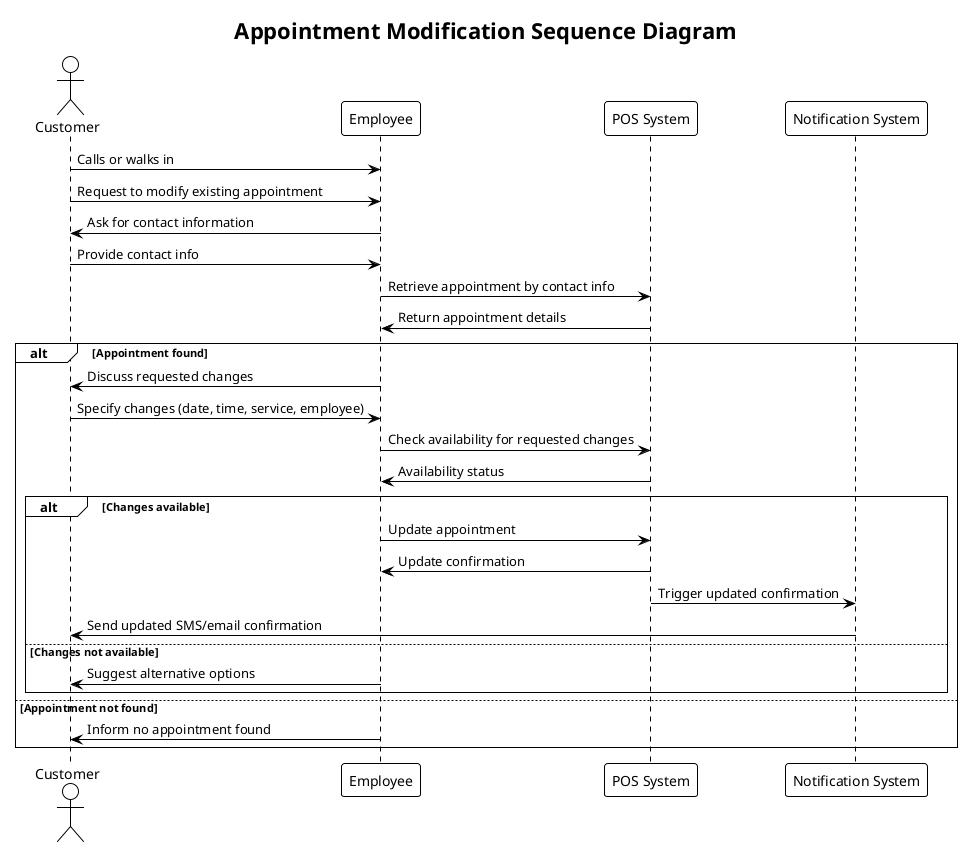
\includegraphics[width=0.8\textwidth]{images/diagrams/services/appointment_modification_sequence.png}
    \caption{Appointment Modification Sequence Diagram}
    \label{fig:appointment_modification_sequence}
\end{figure}

\subsubsection{Cancel appointment business flow}
Flow:
\begin{itemize}
    \setlength{\itemsep}{2pt}
    \setlength{\parskip}{0pt}
    \setlength{\parsep}{0pt}
    \item Customer calls or walks in to the spa/salon
    \item Customer meets with the employee
    \item Customer requests to cancel an existing appointment
    \item Employee asks for customer contact information (phone number, email)
    \item Customer provides contact information
    \item Employee retrieves the appointment using the provided contact information
    \item Employee confirms the cancellation with the customer
    \item Employee cancels the appointment in the POS system
    \item System sends a cancellation confirmation SMS/email to the customer
\end{itemize}

Tables/Entities:
\begin{itemize}
    \setlength{\itemsep}{2pt}
    \setlength{\parskip}{0pt}
    \setlength{\parsep}{0pt}
    \item Customer
    \item Employee
    \item Service
    \item Appointment
    \item Spa/Salon (Business)
\end{itemize}

Components:
\begin{itemize}
    \setlength{\itemsep}{2pt}
    \setlength{\parskip}{0pt}
    \setlength{\parsep}{0pt}
    \item Appointment Management (Appointment, Employee, Service)
    \item Employee Management (Employee)
    \item Notification System (SMS/Email)
\end{itemize}

Actions:
\begin{itemize}
    \setlength{\itemsep}{2pt}
    \setlength{\parskip}{0pt}
    \setlength{\parsep}{0pt}
    \item Retrieve appointment
    \item Cancel appointment
    \item Send cancellation confirmation notification
\end{itemize}

\begin{figure}[H]
    \centering
    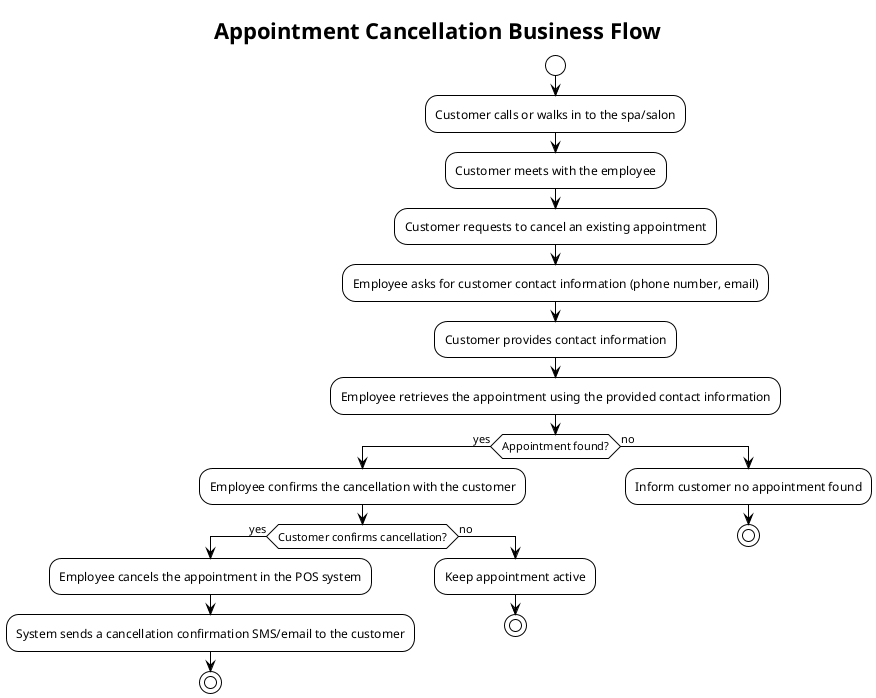
\includegraphics[width=0.8\textwidth]{images/diagrams/services/appointment_cancellation_flow.png}
    \caption{Appointment Cancellation Flow Diagram}
    \label{fig:appointment_cancellation_flow}
\end{figure}

\begin{figure}[H]
    \centering
    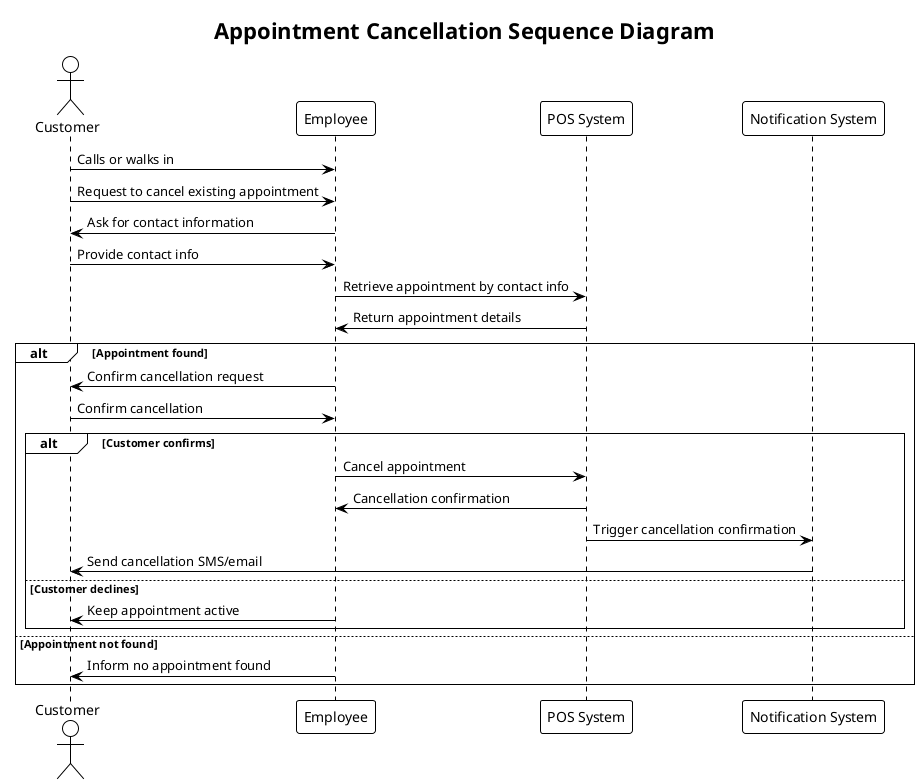
\includegraphics[width=0.8\textwidth]{images/diagrams/services/appointment_cancellation_sequence.png}
    \caption{Appointment Cancellation Sequence Diagram}
    \label{fig:appointment_cancellation_sequence}
\end{figure}


\subsubsection{Service customer business flow}

Flow:
\begin{itemize}
    \setlength{\itemsep}{2pt}
    \setlength{\parskip}{0pt}
    \setlength{\parsep}{0pt}
    \item Customer arrives at the spa/salon for their scheduled appointment
    \item Employee greets the customer and asks customer to confirm their appointment details
    \item Employee verifies the appointment details in the POS system
    \item Employee directs the customer to the appropriate service area and employee
    \item Employee begins providing the scheduled service to the customer
    \item Employee completes the service according to the appointment specifications
    \item Employee asks the customer for the payment method 
    \item Customer provides payment information (cash, card, etc.)
    \item Employee processes the payment in the POS system
    \item System confirms payment and updates the appointment status
    \item Employee asks if the user would like a receipt
    \item If yes, employee prints or emails the receipt to the customer
    \item Customer departs
\end{itemize}

Tables/Entities:
\begin{itemize}
    \setlength{\itemsep}{2pt}
    \setlength{\parskip}{0pt}
    \setlength{\parsep}{0pt}
    \item Customer
    \item Employee
    \item Service
    \item Appointment
    \item Payment
    \item Spa/Salon (Business)
\end{itemize}

Components:
\begin{itemize}
    \setlength{\itemsep}{2pt}
    \setlength{\parskip}{0pt}
    \setlength{\parsep}{0pt}
    \item Appointment Management (Appointment, Service)
    \item Employee Management (Employee)
    \item Payment Processing (Payment)
    \item Notification System (Follow-up notifications)
\end{itemize}

Actions:
\begin{itemize}
    \setlength{\itemsep}{2pt}
    \setlength{\parskip}{0pt}
    \setlength{\parsep}{0pt}
    \item Verify appointment details
    \item Process payment
    \item Mark service as completed
    \item Generate receipt
\end{itemize}

\begin{figure}[H]
    \centering
    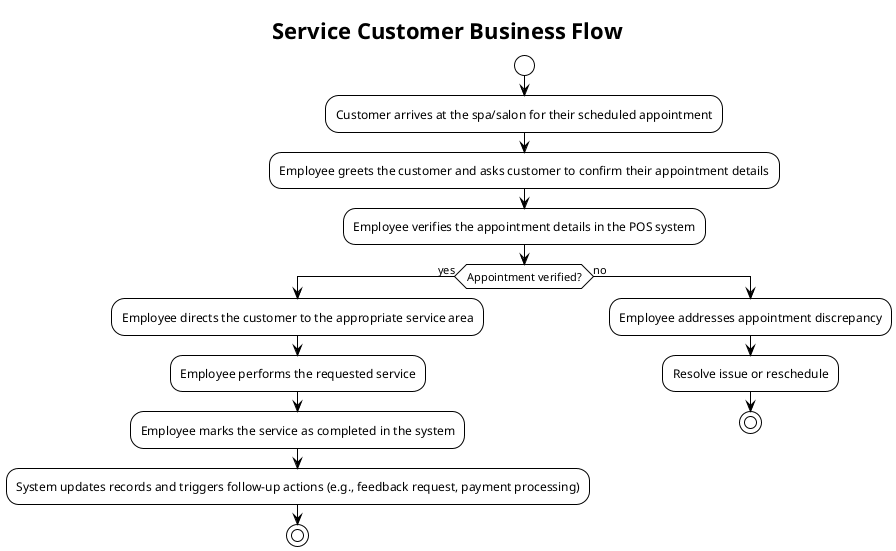
\includegraphics[width=0.8\textwidth]{images/diagrams/services/service_customer_flow.png}
    \caption{Service Customer Flow Diagram}
    \label{fig:service_customer_flow}
\end{figure}

\begin{figure}[H]
    \centering
    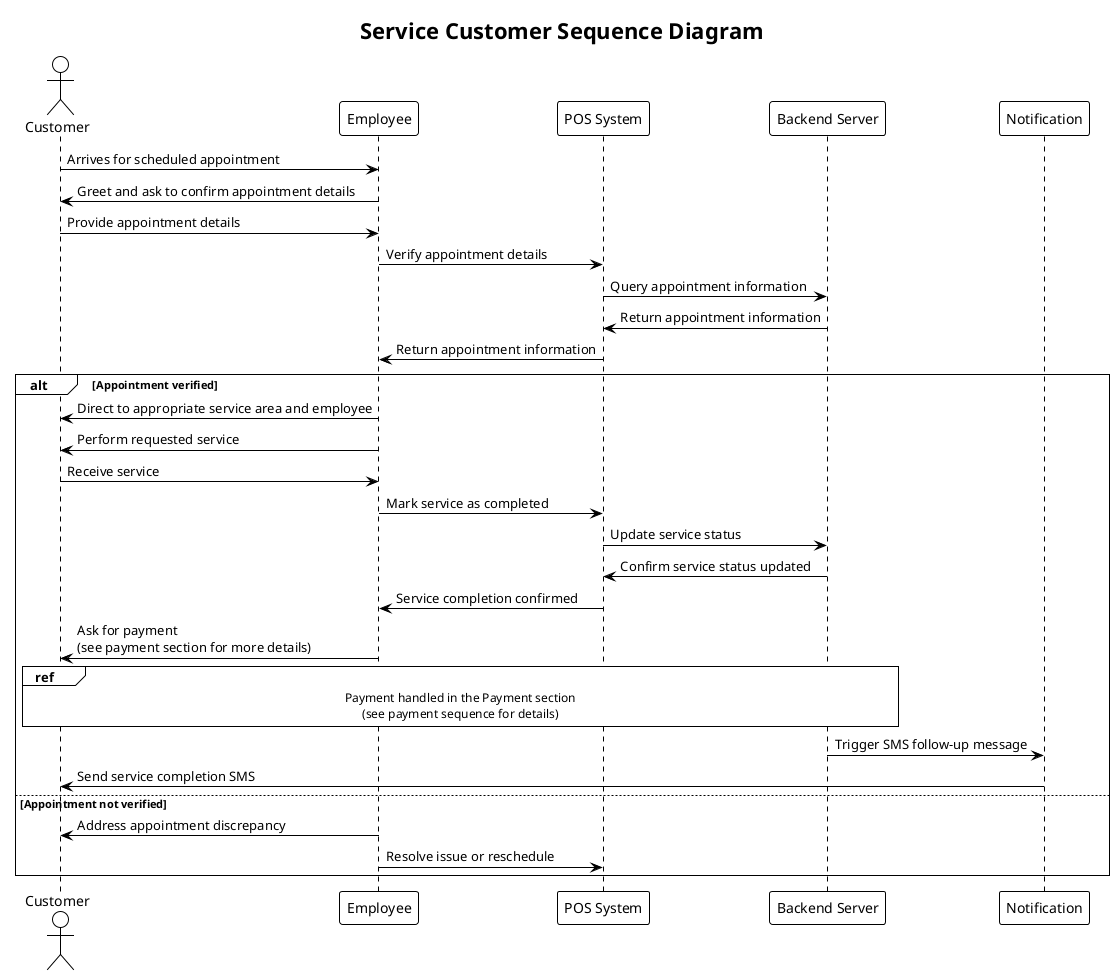
\includegraphics[width=0.8\textwidth]{images/diagrams/services/service_customer_sequence.png}
    \caption{Service Customer Sequence Diagram}
    \label{fig:service_customer_sequence}
\end{figure}

\subsection{Business Management}


% ------------------------------------------------------------------------
% MANAGEMENT DOMAIN (System-wide administrative and operational functions)
% ------------------------------------------------------------------------
% Use Case                           | Description
% ------------------------------------------------------------------------
% User Management                    | Specify business owner can only edit their business's users
% Manage Products/Services           | Add, edit, or deactivate products or services (e.g., menu items, massage types). 
% Manage Product Variations          | Create/edit modifiers for products (e.g., milk type, decaf, size)
% Manage Employees                   | Create, update, or deactivate employee accounts.
% Manage Business Info               | Update business details (owner, address, name, tax ID, contact info).
% Manage Inventory (Optional)        | Track stock levels of items (e.g., ingredients, products).
% Manage Taxes                       | Configure tax rates (e.g., VAT) for different products or services.
% Manage Users & Roles               | Assign permissions to employees (e.g., manager, cashier, admin).
% Super Admin Access                 | Special user (system operator) can access all businesses for support.
% View Reports                       | Generate reports on orders, appointments, revenue, etc.
% Manage Modifiers/Variants          | Define product variants (e.g., latte with almond milk, decaf).
% Manage Discounts                   | Create and manage discount rules (e.g., seasonal, loyalty).
% Manage Service Charges/Tips        | Manage Service Charges/Tips	Configure service charge/gratuity rules (change shouldn't affect historical records)
% Time-Limited Discounts             | Create discounts that are valid only for specific time periods
% ------------------------------------------------------------------------


% ------------------------------------------------------------------------
% Cross-Domain Use Cases (Apply to multiple domains)
% ------------------------------------------------------------------------
% | Use Case                 | Description                                             
% |--------------------------|---------------------------------------------------------
% | Login / Authentication   | Employees log into the system.                          
% | Logout                   | Secure session end.                                     
% | View History             | View past orders or appointments.                       
% | Historical Data Consistency Check   | Ensure changes (e.g., tax updates) don’t affect         
% |                                     | historical records.                                     
% ------------------------------------------------------------------------
We have identified the following Use cases for the Business management domain:

\vspace{1cm}
\begin{longtable}{p{0.25\linewidth} p{0.70\linewidth}}
\caption{Use cases for the Business Management domain} \\
\textbf{Use case} & \textbf{Description} \\
\hline
\endfirsthead

\multicolumn{2}{c}{{\tablename\ \thetable{} -- Continued from previous page}} \\
\textbf{Use case} & \textbf{Description} \\
\hline
\endhead

\multicolumn{2}{c}{{Continued on next page}} \\
\endfoot

\endlastfoot

User Management &
\begin{minipage}[t]{\linewidth}
The business owner can create, update, or deactivate users within their own business. They cannot modify accounts belonging to other businesses.
\end{minipage} \\[6pt]
\multicolumn{2}{@{}c@{}}{\color{gray}\rule{0.95\linewidth}{0.4pt}} \\[6pt]
Manage Products \\ and Services &
\begin{minipage}[t]{\linewidth}
The business owner or authorized staff can add new products/services, edit details (name, price, category), or deactivate them (e.g., coffee, massage type).
\end{minipage} \\[6pt]
\multicolumn{2}{@{}c@{}}{\color{gray}\rule{0.95\linewidth}{0.4pt}} \\[6pt]
Manage Product Variations &
\begin{minipage}[t]{\linewidth}
The business owner or staff can define or edit product modifiers, such as size (small/medium/large), add-ons or other options.
\end{minipage} \\[6pt]
\multicolumn{2}{@{}c@{}}{\color{gray}\rule{0.95\linewidth}{0.4pt}} \\[6pt]
Manage Employees &
\begin{minipage}[t]{\linewidth}
The business owner can create new employee accounts, update employee details (role, contact, availability), or deactivate accounts.
\end{minipage} \\[6pt]
\multicolumn{2}{@{}c@{}}{\color{gray}\rule{0.95\linewidth}{0.4pt}} \\[6pt]
Manage Business Info &
\begin{minipage}[t]{\linewidth}
The business owner can update business details such as the name, address, tax ID, contact information, or ownership information.
\end{minipage} \\[6pt]
\multicolumn{2}{@{}c@{}}{\color{gray}\rule{0.95\linewidth}{0.4pt}} \\[6pt]
Manage Inventory (Optional) &
\begin{minipage}[t]{\linewidth}
The business can track and update stock levels of ingredients or products. System automatically reduces inventory when items are sold, and can alert when stock is low.
\end{minipage} \\[6pt]
\multicolumn{2}{@{}c@{}}{\color{gray}\rule{0.95\linewidth}{0.4pt}} \\[6pt]
Manage Taxes &
\begin{minipage}[t]{\linewidth}
Admins can configure tax rules and rates (e.g., VAT, sales tax) for products or services. Updates affect only new transactions; historical data remains unchanged.
\end{minipage} \\[6pt]
\multicolumn{2}{@{}c@{}}{\color{gray}\rule{0.95\linewidth}{0.4pt}} \\[6pt]
Manage Users \\ and Roles &
\begin{minipage}[t]{\linewidth}
The business owner can assign system roles (manager, cashier, admin, etc.) to employees, controlling access rights and permissions within the system.
\end{minipage} \\[6pt]
\multicolumn{2}{@{}c@{}}{\color{gray}\rule{0.95\linewidth}{0.4pt}} \\[6pt]
Super Admin Access &
\begin{minipage}[t]{\linewidth}
A system operator (Super Admin) can access any business account in the system for technical support, troubleshooting, or emergency fixes.
\end{minipage} \\[6pt]
\multicolumn{2}{@{}c@{}}{\color{gray}\rule{0.95\linewidth}{0.4pt}} \\[6pt]
Manage Modifiers/Variants &
\begin{minipage}[t]{\linewidth}
Admin can define product variants such as “latte with almond milk” or “spa service with aromatherapy add-on.” Variants allow customer customization at order time.
\end{minipage} \\[6pt]
\multicolumn{2}{@{}c@{}}{\color{gray}\rule{0.95\linewidth}{0.4pt}} \\[6pt]
Manage Modifiers/Variants &
\begin{minipage}[t]{\linewidth}
Admin can define product variants such as “latte with almond milk” or “spa service with aromatherapy add-on.” Variants allow customer customization at order timeAdmins can create and manage discount rules (percentage-based, fixed amount, seasonal campaigns, loyalty discounts).
\end{minipage} \\[6pt]
\multicolumn{2}{@{}c@{}}{\color{gray}\rule{0.95\linewidth}{0.4pt}} \\[6pt]
Manage Discounts &
\begin{minipage}[t]{\linewidth}
Admins can create and manage discount rules (percentage-based, fixed amount, seasonal campaigns, loyalty discounts).
\end{minipage} \\[6pt]
\multicolumn{2}{@{}c@{}}{\color{gray}\rule{0.95\linewidth}{0.4pt}} \\[6pt]
Manage Service Charges/Tips &
\begin{minipage}[t]{\linewidth}
Admins can configure rules for applying service charges or gratuities. Updates only apply to future transactions, ensuring historical data remains intact.
\end{minipage} \\[6pt]
\multicolumn{2}{@{}c@{}}{\color{gray}\rule{0.95\linewidth}{0.4pt}} \\[6pt]
Time-Limited Discounts &
\begin{minipage}[t]{\linewidth}
Admins can create discounts restricted to a specific timeframe (e.g., happy hour, seasonal promotions). The system enforces validity automatically.
\end{minipage} \\[6pt]
\multicolumn{2}{@{}c@{}}{\color{gray}\rule{0.95\linewidth}{0.4pt}} \\[6pt]

\end{longtable}

We have identified the following Cross-Domain Use cases for the Business management domain:
\vspace{1cm}
\begin{longtable}{p{0.25\linewidth} p{0.70\linewidth}}
\caption{Cross-Domain Use cases for the Business Management domain} \\
\textbf{Use case} & \textbf{Description} \\
\hline
\endfirsthead

\multicolumn{2}{c}{{\tablename\ \thetable{} -- Continued from previous page}} \\
\textbf{Use case} & \textbf{Description} \\
\hline
\endhead

\multicolumn{2}{c}{{Continued on next page}} \\
\endfoot

\endlastfoot

Login / Authentication &
\begin{minipage}[t]{\linewidth}
Employees log into the system using their credentials. The system validates identity and assigns permissions based on role.
\end{minipage} \\[6pt]
\multicolumn{2}{@{}c@{}}{\color{gray}\rule{0.95\linewidth}{0.4pt}} \\[6pt]
Logout &
\begin{minipage}[t]{\linewidth}
Employees securely end their session. The system clears active tokens/sessions and confirms logout Users (customers, employees, or admins) can view past orders, appointments, or reports. This ensures transparency and auditability.
\end{minipage} \\[6pt]
\multicolumn{2}{@{}c@{}}{\color{gray}\rule{0.95\linewidth}{0.4pt}} \\[6pt]
View Historical Data, Consistency Check &
\begin{minipage}[t]{\linewidth}
Users (customers, employees, or admins) can view past orders, appointments, or reports. This ensures transparency and auditability.
\end{minipage} \\[6pt]
\multicolumn{2}{@{}c@{}}{\color{gray}\rule{0.95\linewidth}{0.4pt}} \\[6pt]
Historical Data Consistency Check &
\begin{minipage}[t]{\linewidth}
The system ensures that administrative changes (tax rates, discounts, service charges) apply only to new transactions, without modifying historical order or appointment records.
\end{minipage} \\[6pt]
\multicolumn{2}{@{}c@{}}{\color{gray}\rule{0.95\linewidth}{0.4pt}} \\[6pt]

\end{longtable}
\setcounter{secnumdepth}{5}
\subsubsection{User \& Role Management}
% related use cases: User Management, Manage Employees, Manage Users & Roles, Super Admin Access

\paragraph{User Management}
% Need to better think of what components and entities are involved and their names
\begin{itemize}
    \item \textbf{Flow}: \begin{enumerate}
    \item Owner selects "Manage Users"
    \item Owner creates/updates/deletes a user.
    \item System validates ownership (can only edit their business).
    \item System updates User Table.
    \item System confirms operation.
    \end{enumerate}
    \item \textbf{Entities}: Owner, User System, Backend Server, User DB.
    \item \textbf{Components \& Actions}: \begin{itemize}
        \item UI (input user details / User System).
        \item Auth Service (ownership validation).
        \item User Service (CRUD operations)
    \end{itemize}
\end{itemize}

\paragraph{Manage Employees}

\begin{itemize}
    \item \textbf{Flow}: \begin{enumerate}
    \item Owner selects "Employees".
    \item Owner creates/updates/deactivates employee account.
    \item System validates uniqueness.
    \item System updates Employee table.
    \item System sends confirmation.
    \end{enumerate}
    \item \textbf{Entities}: Owner, Employee System, Backend Server, Employee DB.
    \item \textbf{Components \& Actions}: \begin{itemize}
        \item Employee Service (input employee details).
        \item Auth Service (restrict to owner).
    \end{itemize}
\end{itemize}

\paragraph{Manage Users \& Roles}

\begin{itemize}
    \item \textbf{Flow}: \begin{enumerate}
    \item Owner selects "Roles".
    \item Assigns role to employee (e.g. cashier).
    \item System validates role assignment.
    \item System updates Employee Roles table.
    \item System confirms operation.
    \end{enumerate}
    \item \textbf{Entities}: Owner, Employee System, Backend Server, Role DB.
    \item \textbf{Components \& Actions}: \begin{itemize}
        \item Role Service.
        \item Auth Service (restrict to owner).
    \end{itemize}
\end{itemize}

\paragraph{Super Admin Access}

\begin{itemize}
    \item \textbf{Flow}: \begin{enumerate}
    \item Super Admin logs in.
    \item Selects business.
    \item Views/edits users, settings.
    \item System validates elevated permissions.
    \item System updates relevant tables.
    \end{enumerate}
    \item \textbf{Entities}: Super Admin, System, Backend Server, User DB.
    \item \textbf{Components \& Actions}: \begin{itemize}
        \item Auth Service (restrict to owner).
        \item User/Business Service.
    \end{itemize}
\end{itemize}

\subsubsection{Product \& Service Management}
% related use cases: Manage Products/Services, Manage Product Variations, Manage Modifiers, Variants
\paragraph{Manage Products/Services}

\begin{itemize}
    \item \textbf{Flow}: \begin{enumerate}
    \item Owner selects "Products/Services"..
    \item Owner adds/edits/deactivates an item.
    \item System validates input.
    \item System updates Product/Service table.
    \item System confirms update.
    \end{enumerate}
    \item \textbf{Entities}: Owner, System, Product/Service DB.
    \item \textbf{Components \& Actions}: \begin{itemize}
        \item Product Service (create/edit/deactivate).
        \item Validation Service (ensure valid fields).
    \end{itemize}
\end{itemize}

\paragraph{Manage Product Variations}

\begin{itemize}
    \item \textbf{Flow}: \begin{enumerate}
    \item Owner selects product.
    \item Adds/modifies variation.
    \item System validates variation rules.
    \item System updates Product\_Variation table.
    \item System confirms update.
    \end{enumerate}
    \item \textbf{Entities}: Owner, System, Product DB, Variation DB.
    \item \textbf{Components \& Actions}: \begin{itemize}
        \item Variation Manager.
        \item Validation Service.
    \end{itemize}
\end{itemize}

\paragraph{Manage Modifiers/Variants}

\begin{itemize}
    \item \textbf{Flow}: \begin{enumerate}
    \item Owner selects product.
    \item Defines variant.
    \item System validates rules.
    \item System updates Variant table.
    \item System confirms update.
    \end{enumerate}
    \item \textbf{Entities}: Owner, System, Product DB, Variation DB.
    \item \textbf{Components \& Actions}: \begin{itemize}
        \item Variation Manager.
        \item Validation Service.
    \end{itemize}
\end{itemize}



\subsubsection{Business \& Information Management}
% related use cases: Manage Business Info
\subsubsection{Inventory \& Taxes}
% related use cases: Manage Inventory (Optional), Manage Taxes
\subsubsection{Discounts \& Charges}
% related use cases: Manage Discounts, Time-Limited Discounts, ips
\subsubsection{Reports}
% related use cases: View Reports

\subsubsection{Cross-Domain}
% related use cases: Login / Authentication, Logout, View History, Historical Data Consistency Check


\printbibliography[title = {References and sources}]

\end{document}
